\chapter{End of Life Reactivity} \label{ch:sweeps}
A valid reactor design must meet certain neutronics constraints. The main
neutronics constraint is reactivity. The reactor must be able to sustain a chain
reaction from startup, to the final second of the 10 year lifetime. End of Life
(EOL) reactivity was the target metric for the neutronic design of the core.
Traditional reactor design processes will spend a long time tweaking neutronics
parameters to meet certain system performances. The total mass optimization
needed a rapidly excecutable model that could respond to various inputs.
This need meant it was important to understand how a reactor's neutronic
performance is impacted by various input and design parametres. An n-dimensional 
sampling was performed to explore EOL \keff dependence on various reactor parameters.

\section{Parametric Study of Neutronics Parameters}
Homogeneous MCNP6.1 depletion models were used to analyze the EOL \keff response
to neutronics parameters (predictors). The core region was homogenized and
surrounded by a graphite reflector. A large set of 5-dimensional predictors and
EOL \keff results was produced to investigate the neutronics parameter space.
These predictors and their results helped develop an understanding of the
reactor response to important design and operational parameters. High Throughput
Computing capabilities at UW were used to perform 3901 depletion calculations
with MCNP6.1. Each model represents a unique sampling in every dimension using
the Latin Hypercube Sampling (LHS) technique\citep{LHS}. The LHS technique ensured even
sampling for every dimension. The sampled and fixed dimensions/parameters are
shown in Table \ref{tab:lhs_sweep_vars}.

\begin{table}[h]
  \centering
  \caption{Homogeneous Geometry and Depletion Parameters}
  \begin{tabular}{ll}
    \toprule
     Core Radius                		   & 10 - 50 [cm] \\
     Fuel Enrichment 					   & 20\% - 90\% $^{235}$U\\
     Reflector Thickness				   & 15 [cm]\\
     Coolant Channel Radius                & 0.5 - 1 [cm] \\
     Fuel Pitch to Coolant Channel D.      & 1.1-1.6 [-]\\
     Thermal Power						   & 80-200 [kW]\\
     Core Aspect Ratio					   & 1 [-] \\
     Fuel Temp  						   & 300 [K]\\
     Reactor Physics Code, Data			   & MCNP6.1, ENDF-7.2
  \end{tabular}
  \label{tab:lhs_sweep_vars}
\end{table}

\section{Parametric Study Results}
The target metric for the neutronics sampling was an EOL \keff equal to one. In
order to determine the dependence of EOL \keff on each swept parameter in Table
\ref{tab:lhs_sweep_vars}, EOL \keff was plotted against the parameters.

\subsection{Core Radius}
Fuel mass is the strongest predictor of EOL \keff. As a result, core radius has a strong impact on EOL \keff. Fuel mass is directly correlated
to fuel fraction and core volume. For a fixed aspect ratio of 1, core volume is
a cubic function of core radius. This makes EOL \keff strongly dependent on core
radius. The volume to surface area ratio is a positive function of core radius
hence, neutron leakge is reduced in larger cores. 

\begin{figure}[h]
    \centering
    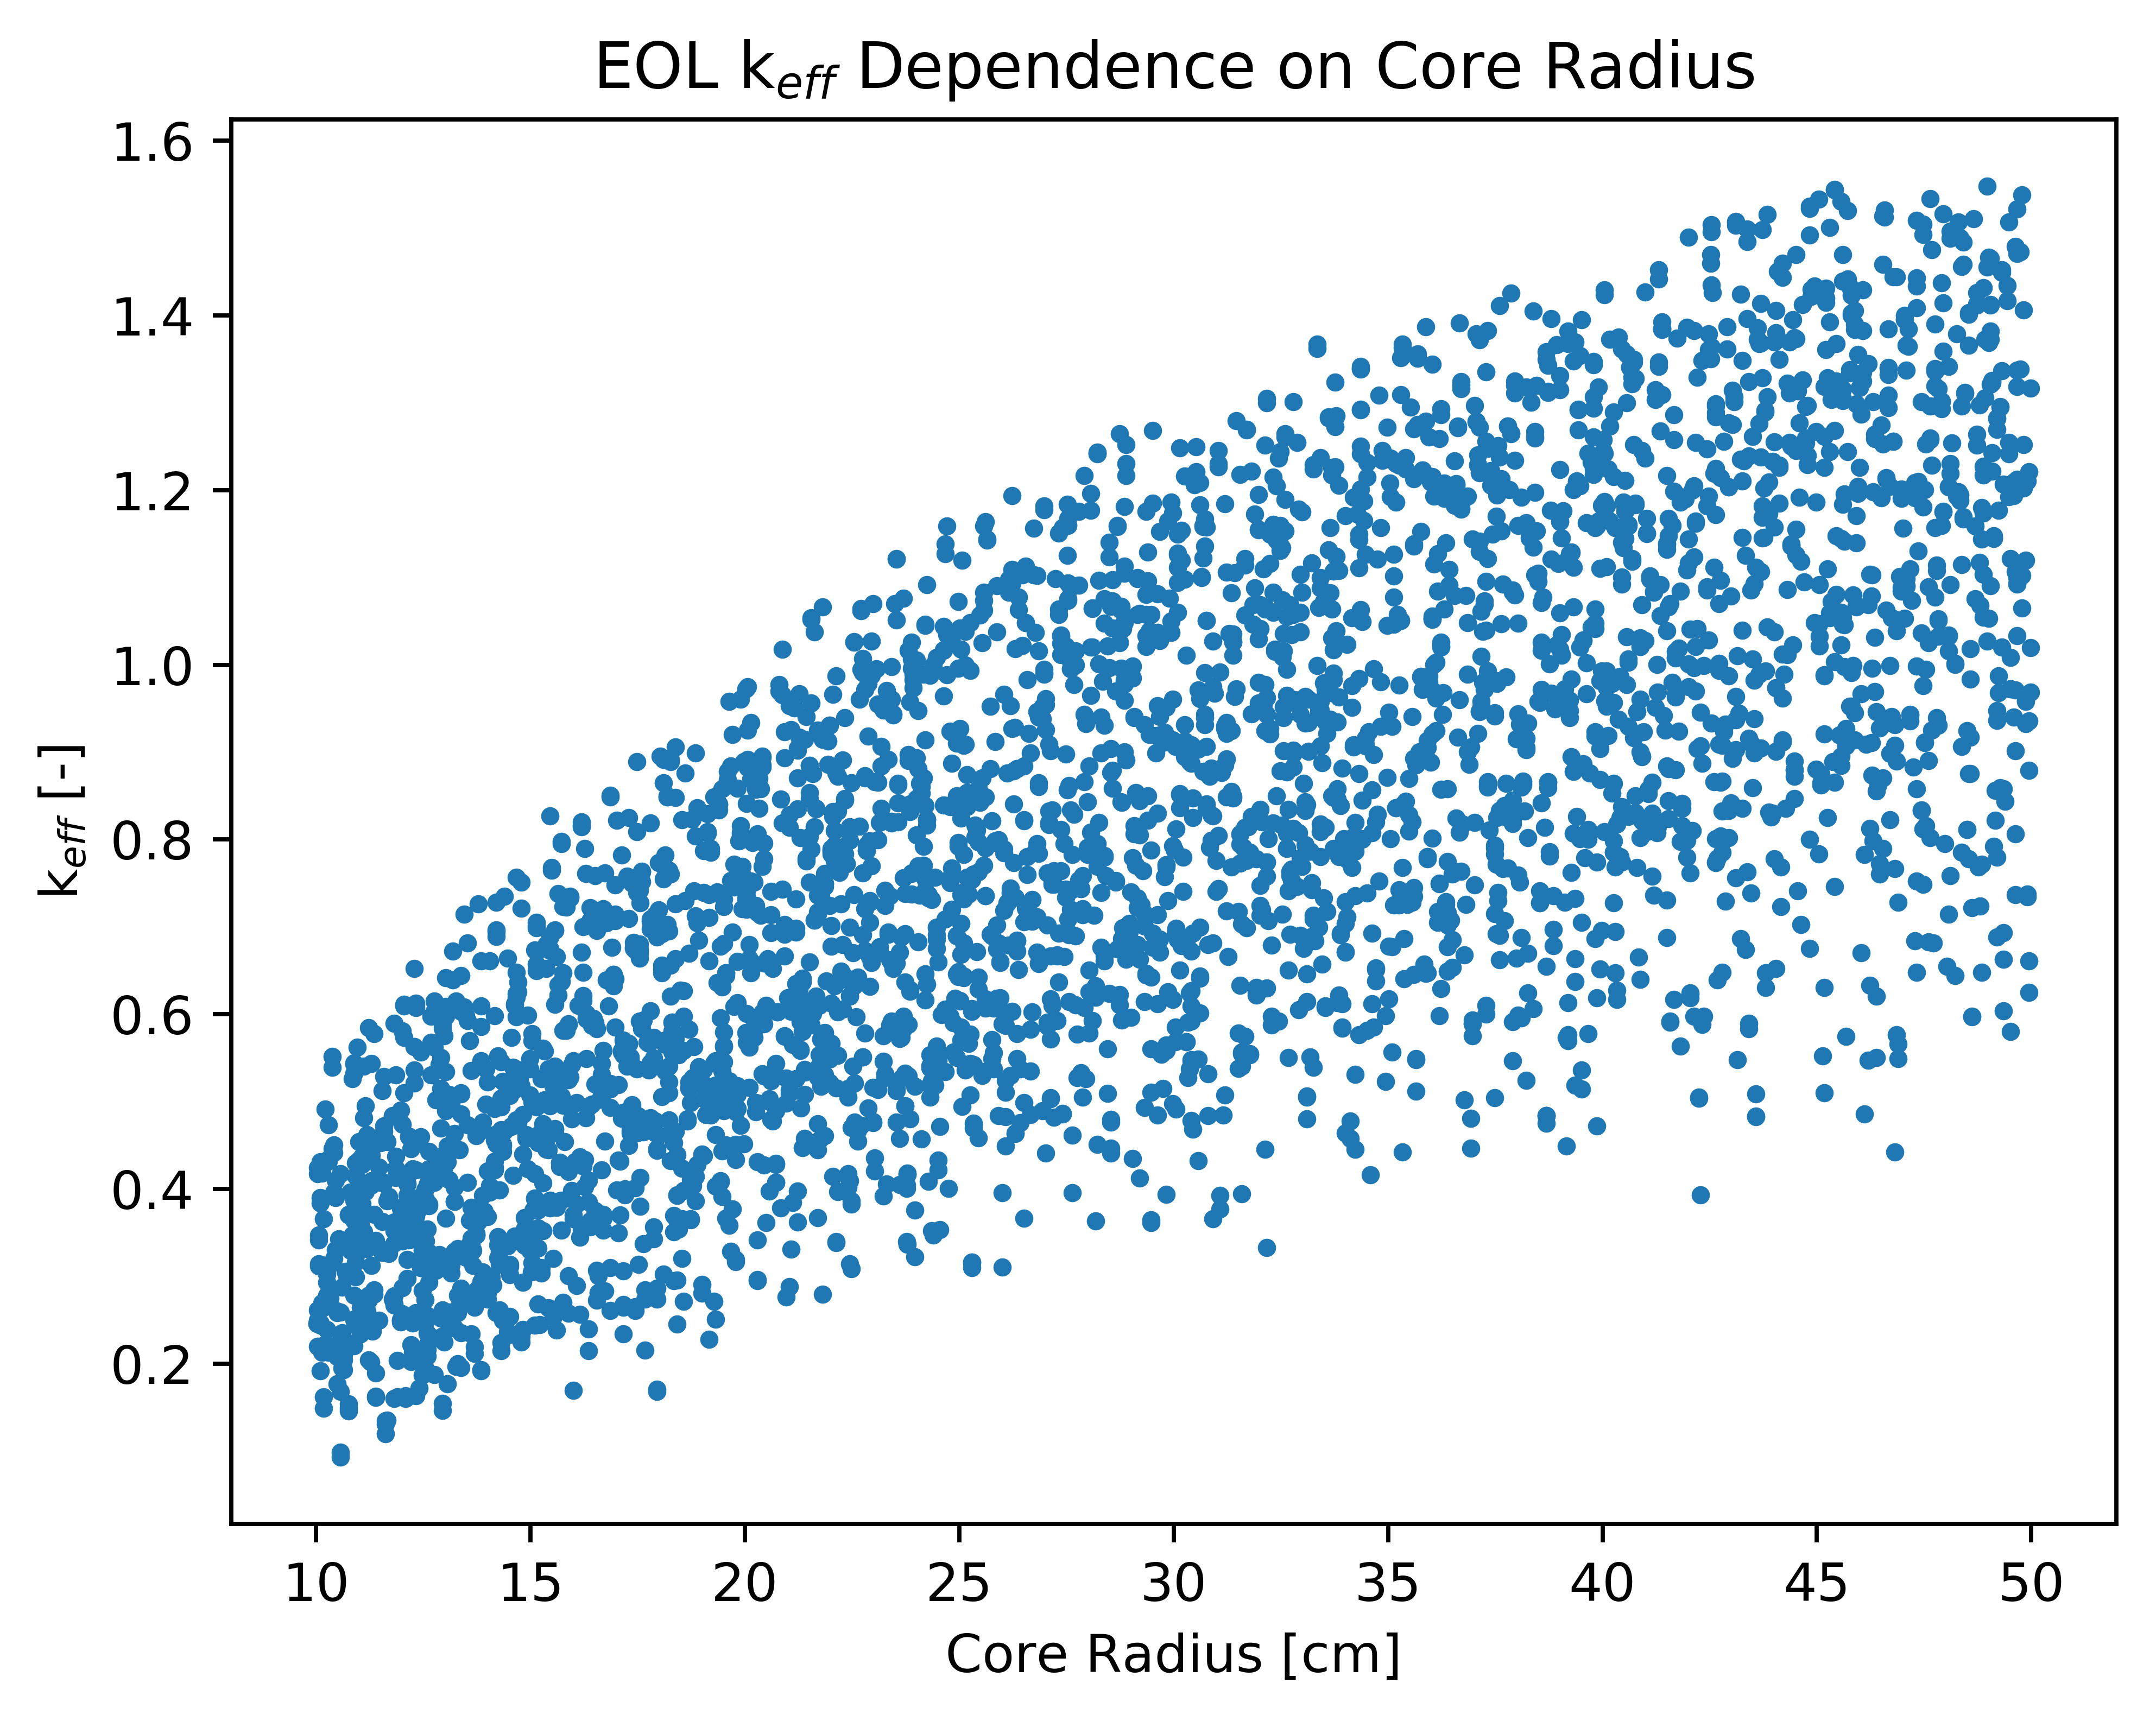
\includegraphics[width=3in]{../images/keff_vs_core_r.png}
\caption{EOL \keff dependence on core radius.}
\label{fig:eol_keff_vs_r_core}
\end{figure}

\subsection{Fuel Enrichment}
EOL \keff is directly dependent on fuel enrichment. Mass of \uran is the most
important metric to predict EOL \keff. Figure
\ref{fig:eol_keff_vs_mass_enrich} shows the result of the enrichment sweep in the context of
fuel mass dependence, reducing core radius and fuel pitch to channel diameter to
one metric, total fuel mass. The colorbar shows the impact of enrichment. For a fixed core
mass, increasing enrichment leads to increasing EOL \keff. 

\begin{figure}[h]
    \centering
    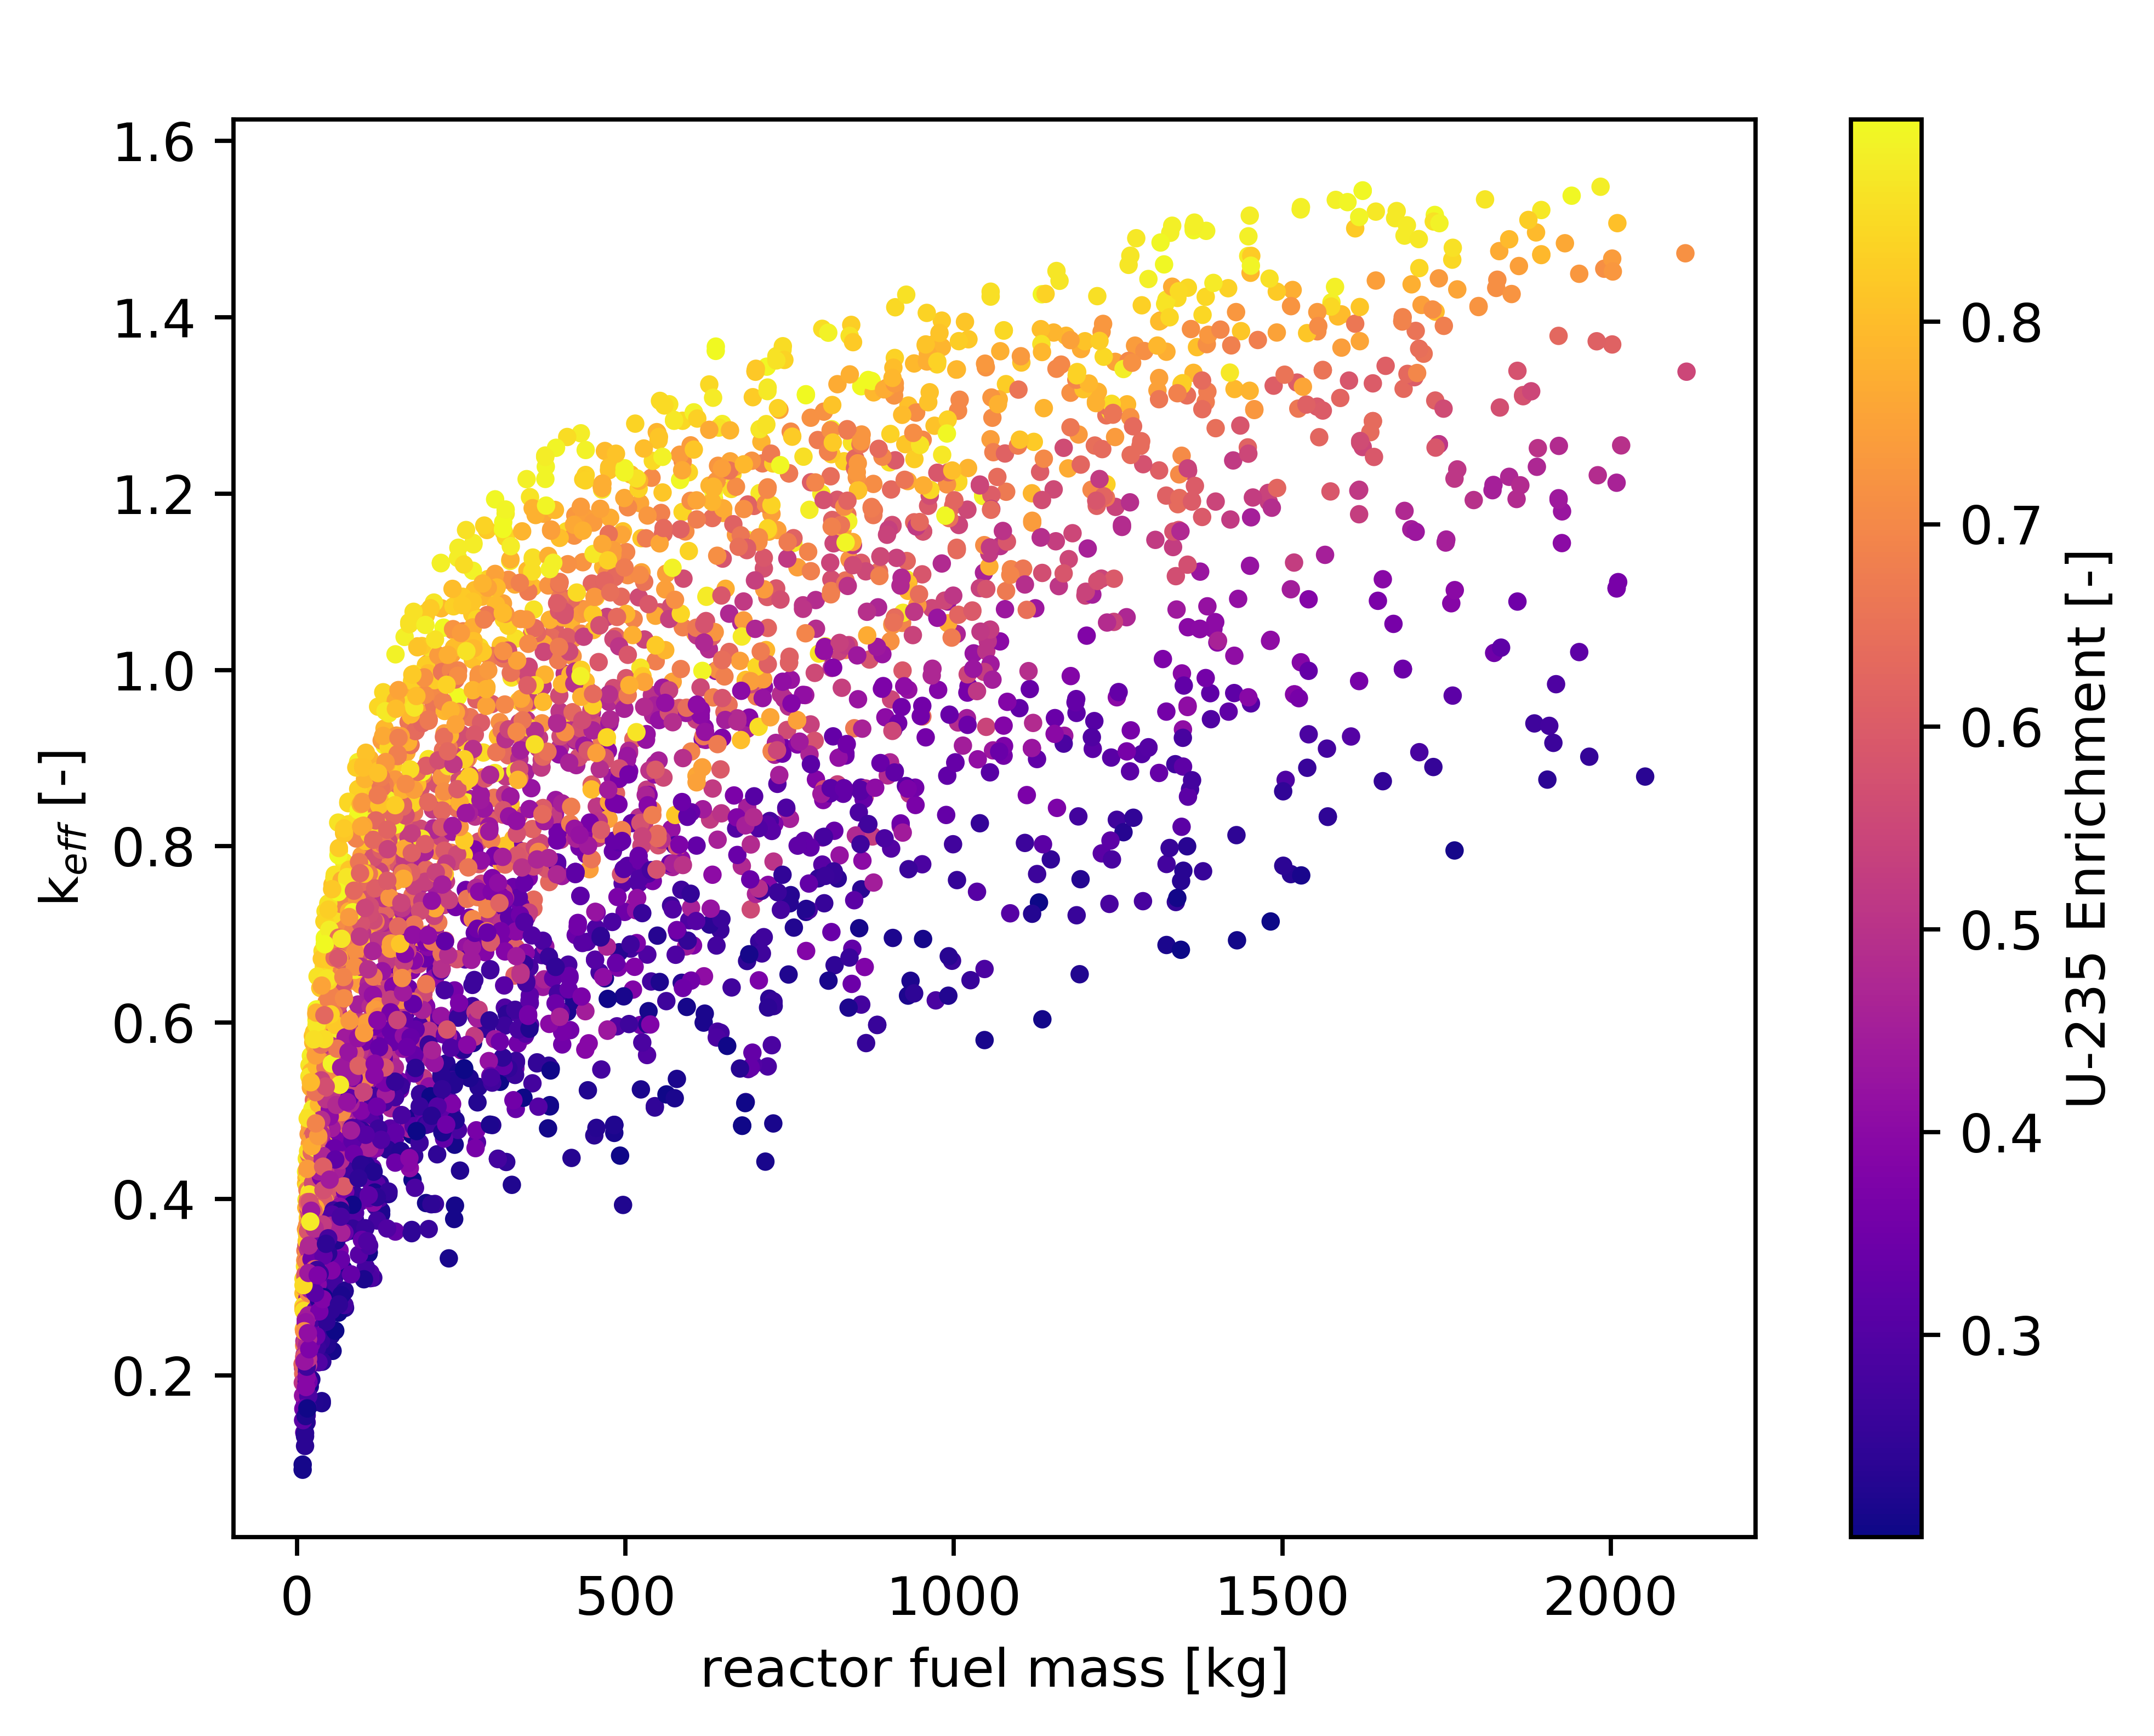
\includegraphics[width=3in]{../images/keff_vs_mass_enrich.png}
\caption{EOL \keff dependence on fuel enrichment}
\label{fig:eol_keff_vs_mass_enrich}
\end{figure}


\subsection{Coolant Channel Radius}
EOL \keff is independent of coolant channel radius. Small geometric features
have little importance for high energy reactors. Figure
\ref{fig:eol_keff_vs_r_cool} shows the result of this sweep.

\begin{figure}[h]
    \centering
    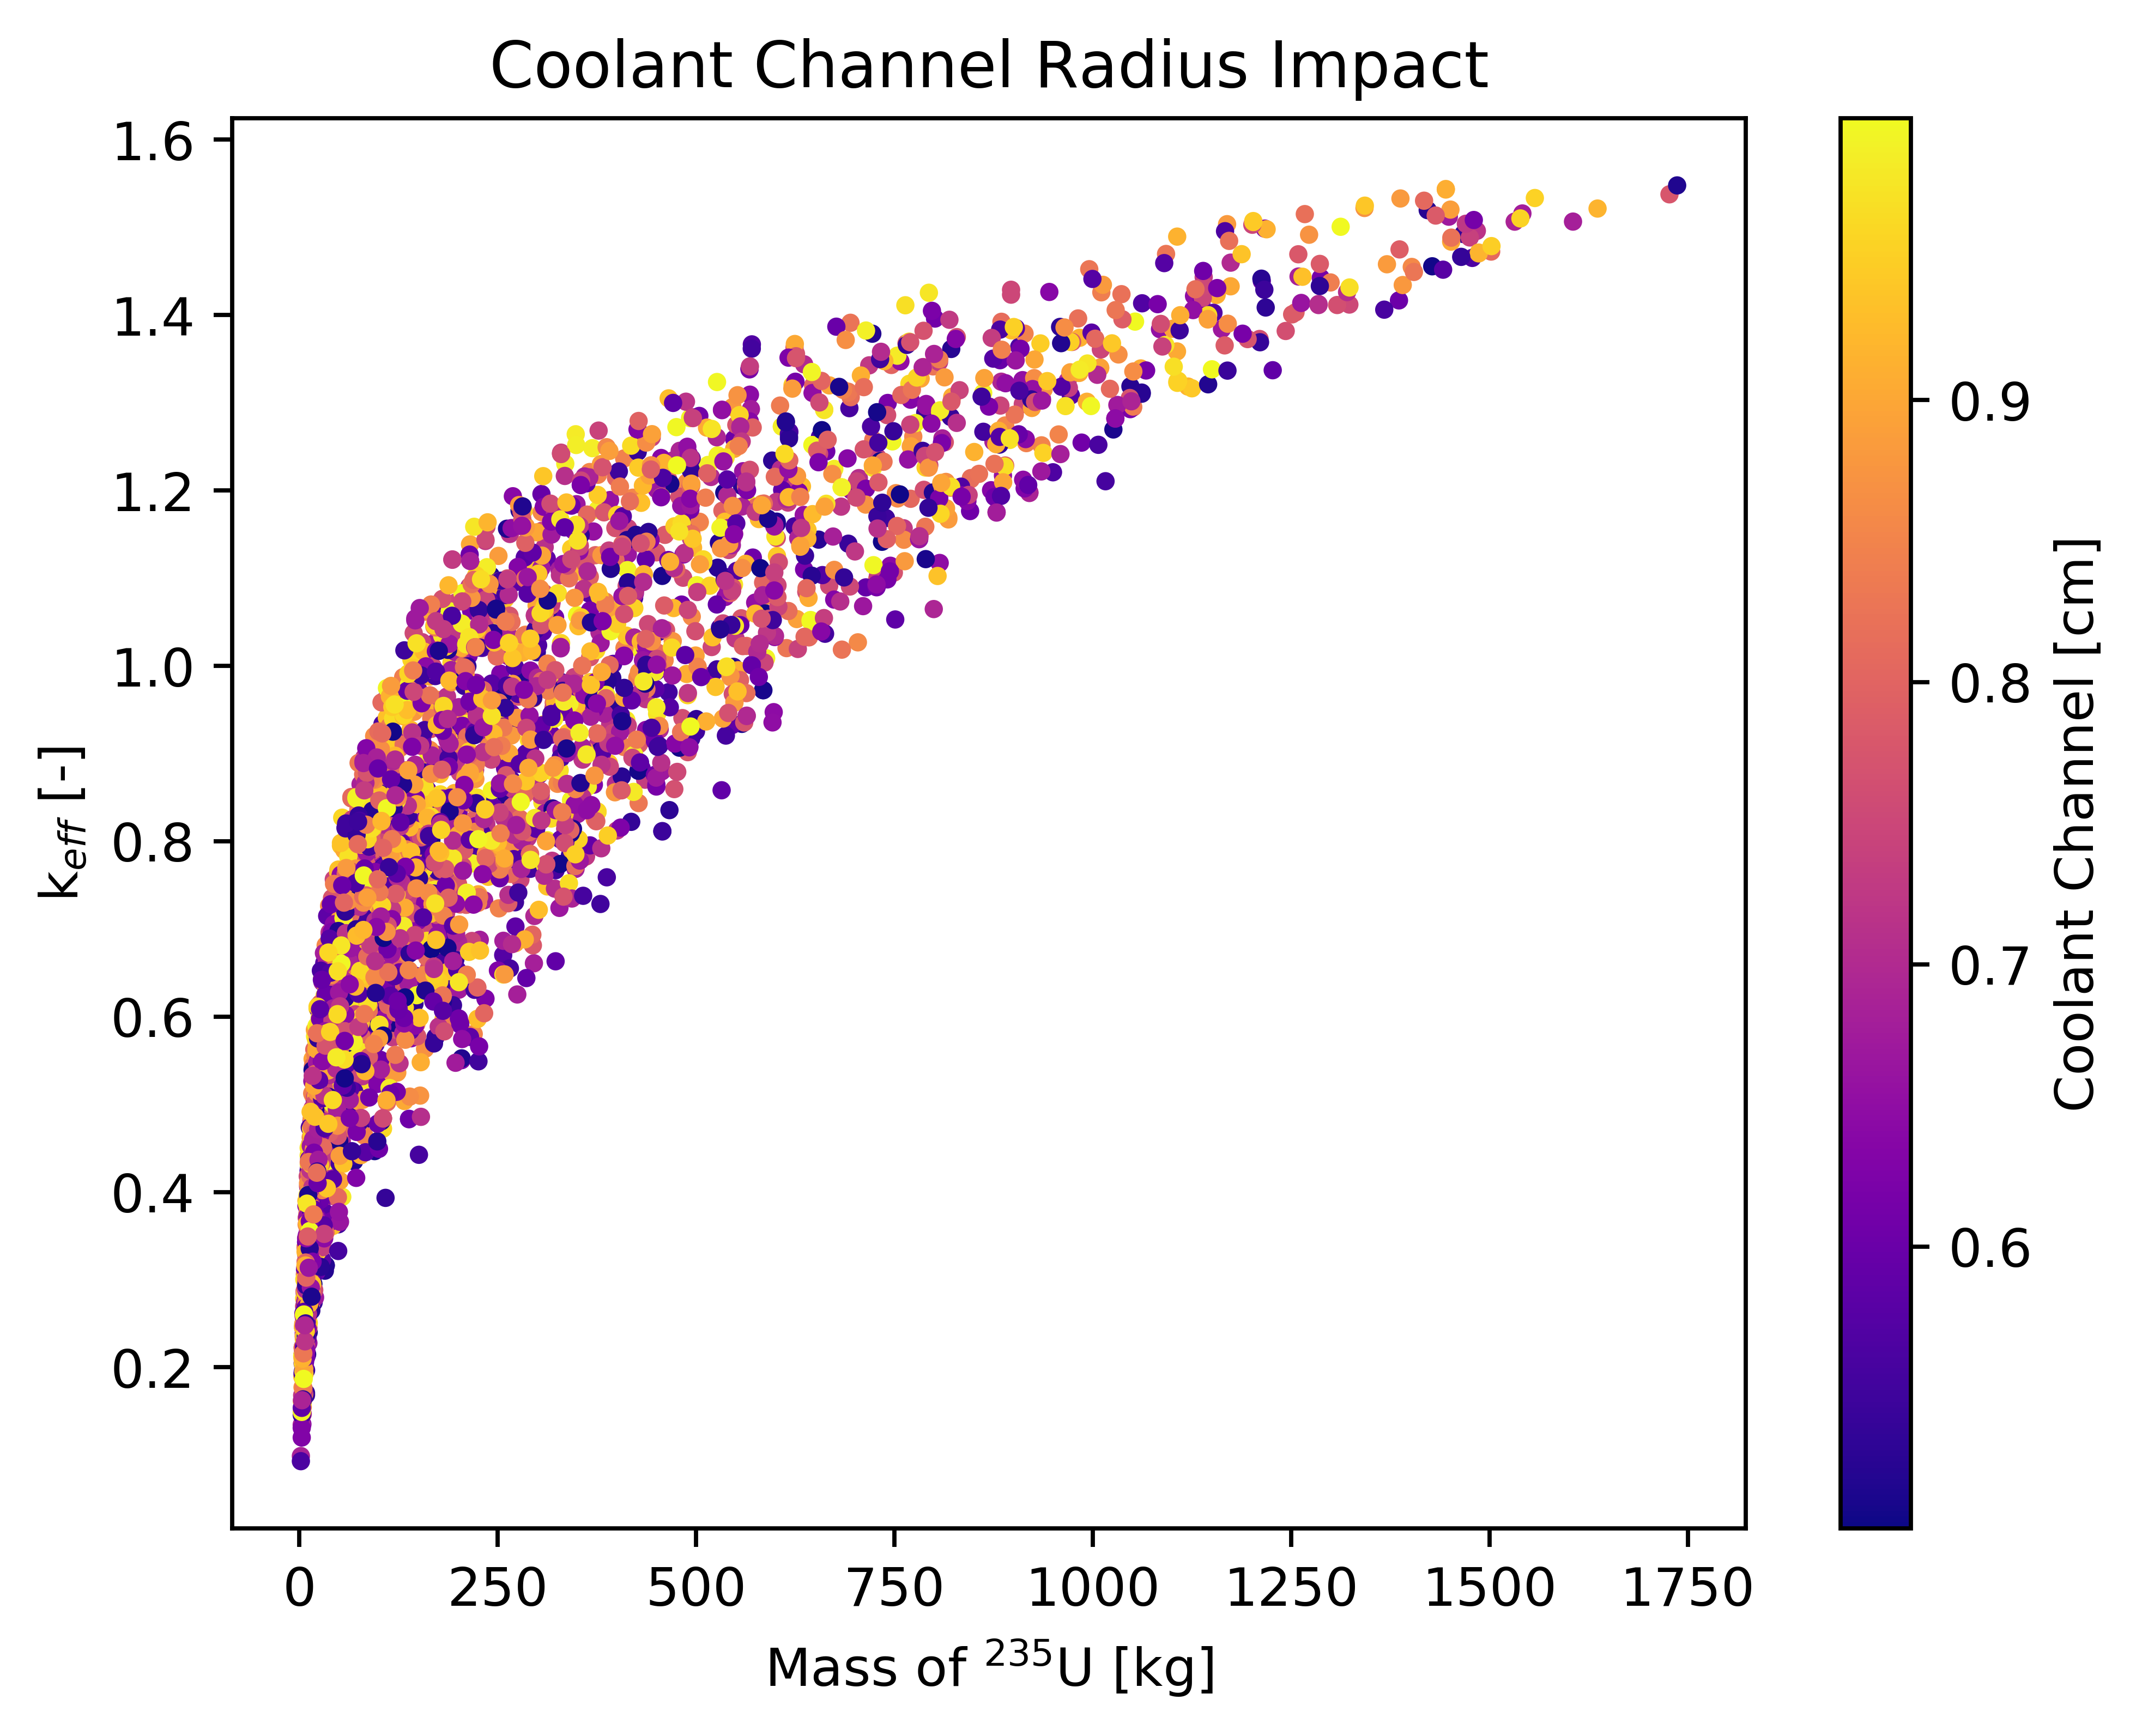
\includegraphics[width=3in]{../images/keff_vs_cool_r.png}
\caption{EOL \keff dependence on coolant channel radius}
\label{fig:eol_keff_vs_r_cool}
\end{figure}

\subsection{Fuel Pitch to Coolant Channel Diameter}
Fuel pitch to coolant channel diameter was used as the inverse of the traditional pitch
to diameter ratio in power reactors. The inverted fuel configuration with
coolant flowing through the middle of a fuel block motivated this metric. Like
core radius, PD impacts EOL \keff by dictating fuel mass. The high-energy
neutron spectrum means the geometric features have a small impact on the
neutronics of the reactor. A large PD yields a large fuel fraction and as a
result, a large fuel mass. Figure
\ref{fig:eol_keff_vs_PD_mass} shows the result of this sweep, with the colorbar
showing total fuel mass.

\begin{figure}[h]
    \centering
    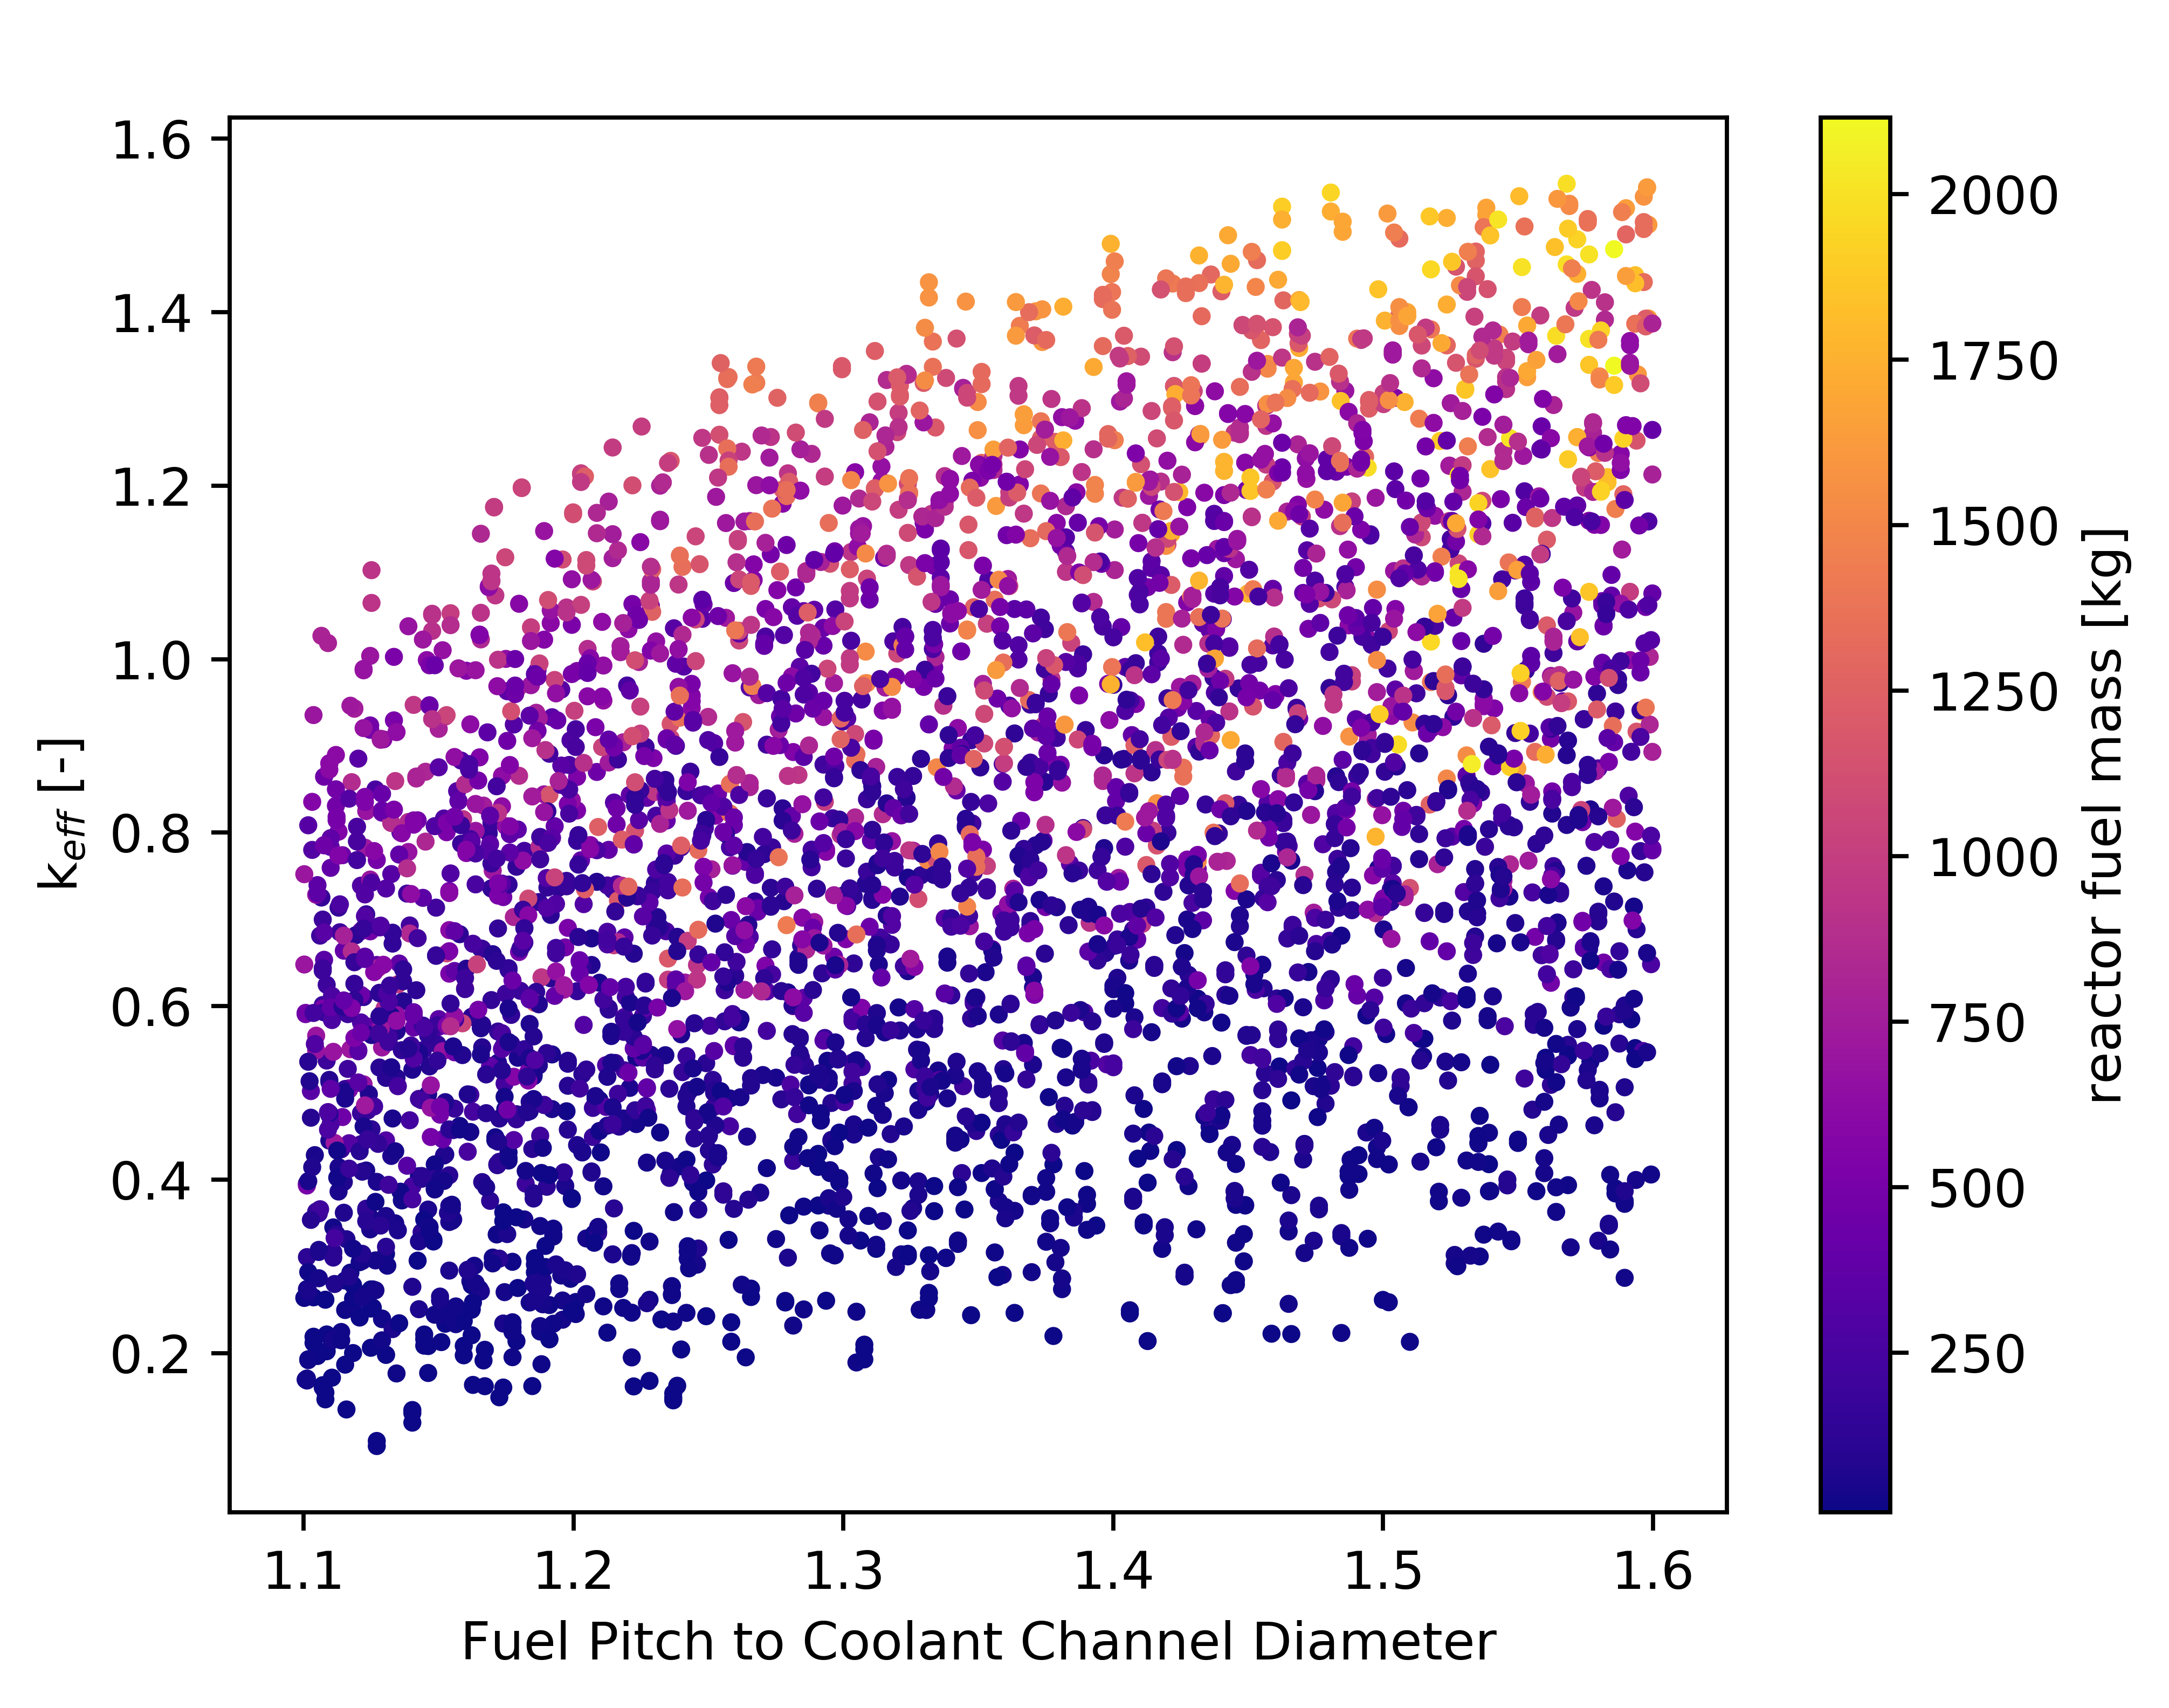
\includegraphics[width=3in]{../images/keff_vs_PD_mass.png}
\caption{EOL \keff dependence on fuel pitch to coolant channel ratio}
\label{fig:eol_keff_vs_PD_mass}
\end{figure}


\subsection{Thermal Power}
Initially, the result of greatest interest was the mass dependence on thermal
power because thermal power was the reactor-power cycle coupling parameter.
Figure \ref{fig:eol_keff_vs_power} shows the relationship between thermal power
and EOL \keff.

\begin{figure}[h]
    \centering
    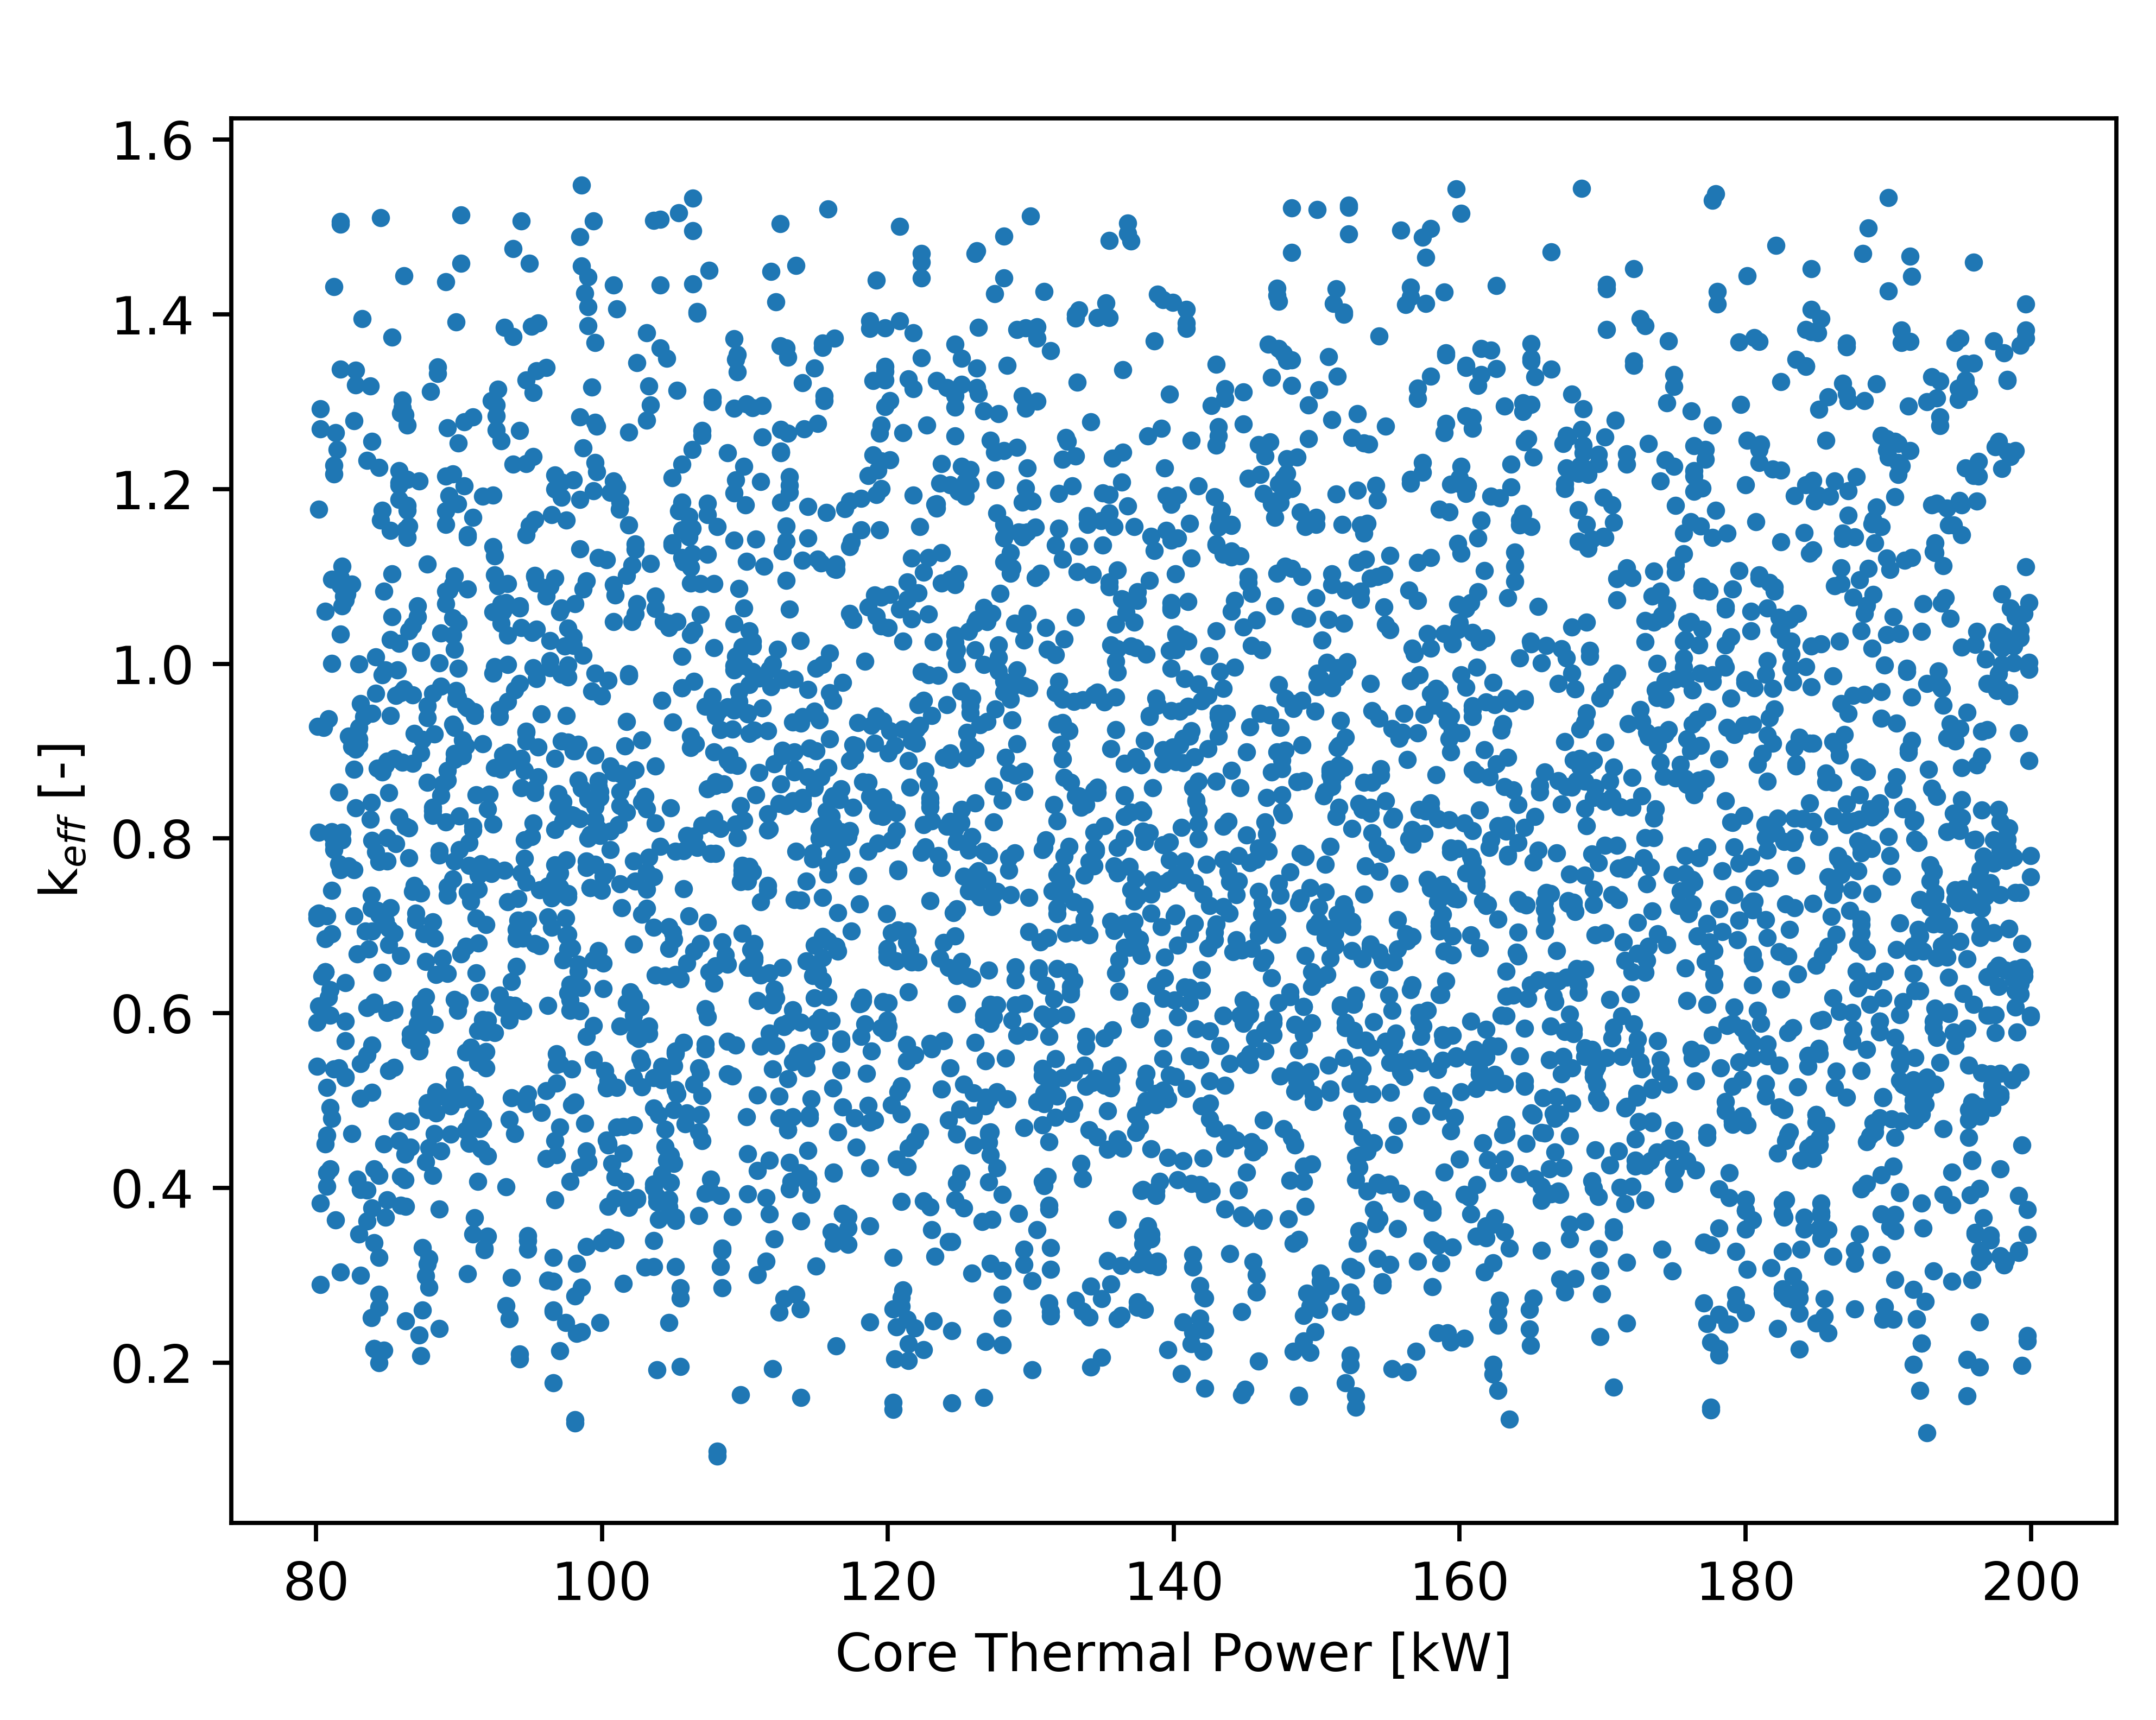
\includegraphics[width=3in]{../images/keff_vs_power.png}
\caption{EOL \keff dependence on thermal power}
\label{fig:eol_keff_vs_power}
\end{figure}

As shown in Figure \ref{fig:eol_keff_vs_power}, EOL \keff is independent of core
thermal power. This result is not surprising considering the depletion rates in
the core. Assuming 1 MWd/gU is an achievable burnup, the reactor depletes
approximately 1000 g of uranium over 10 years of full power operation (at 200
kW). The depletion mass
of uranium is negligigle compared to the mass of uranium required for the
reactor to be critical at BOL. Thermal power is not a strong predictor of EOL
criticality.

\subsection{Uranium 235 Mass}
The strongest predictor of EOL \keff is a combination of some of the above
swept parameters. The most important metric for EOL \keff is the mass of \uran
in the system. Figure \ref{fig:eol_keff_vs_235_mass} shows the dependence of EOL
\keff on \uran mass.

\begin{figure}[h]
    \centering
    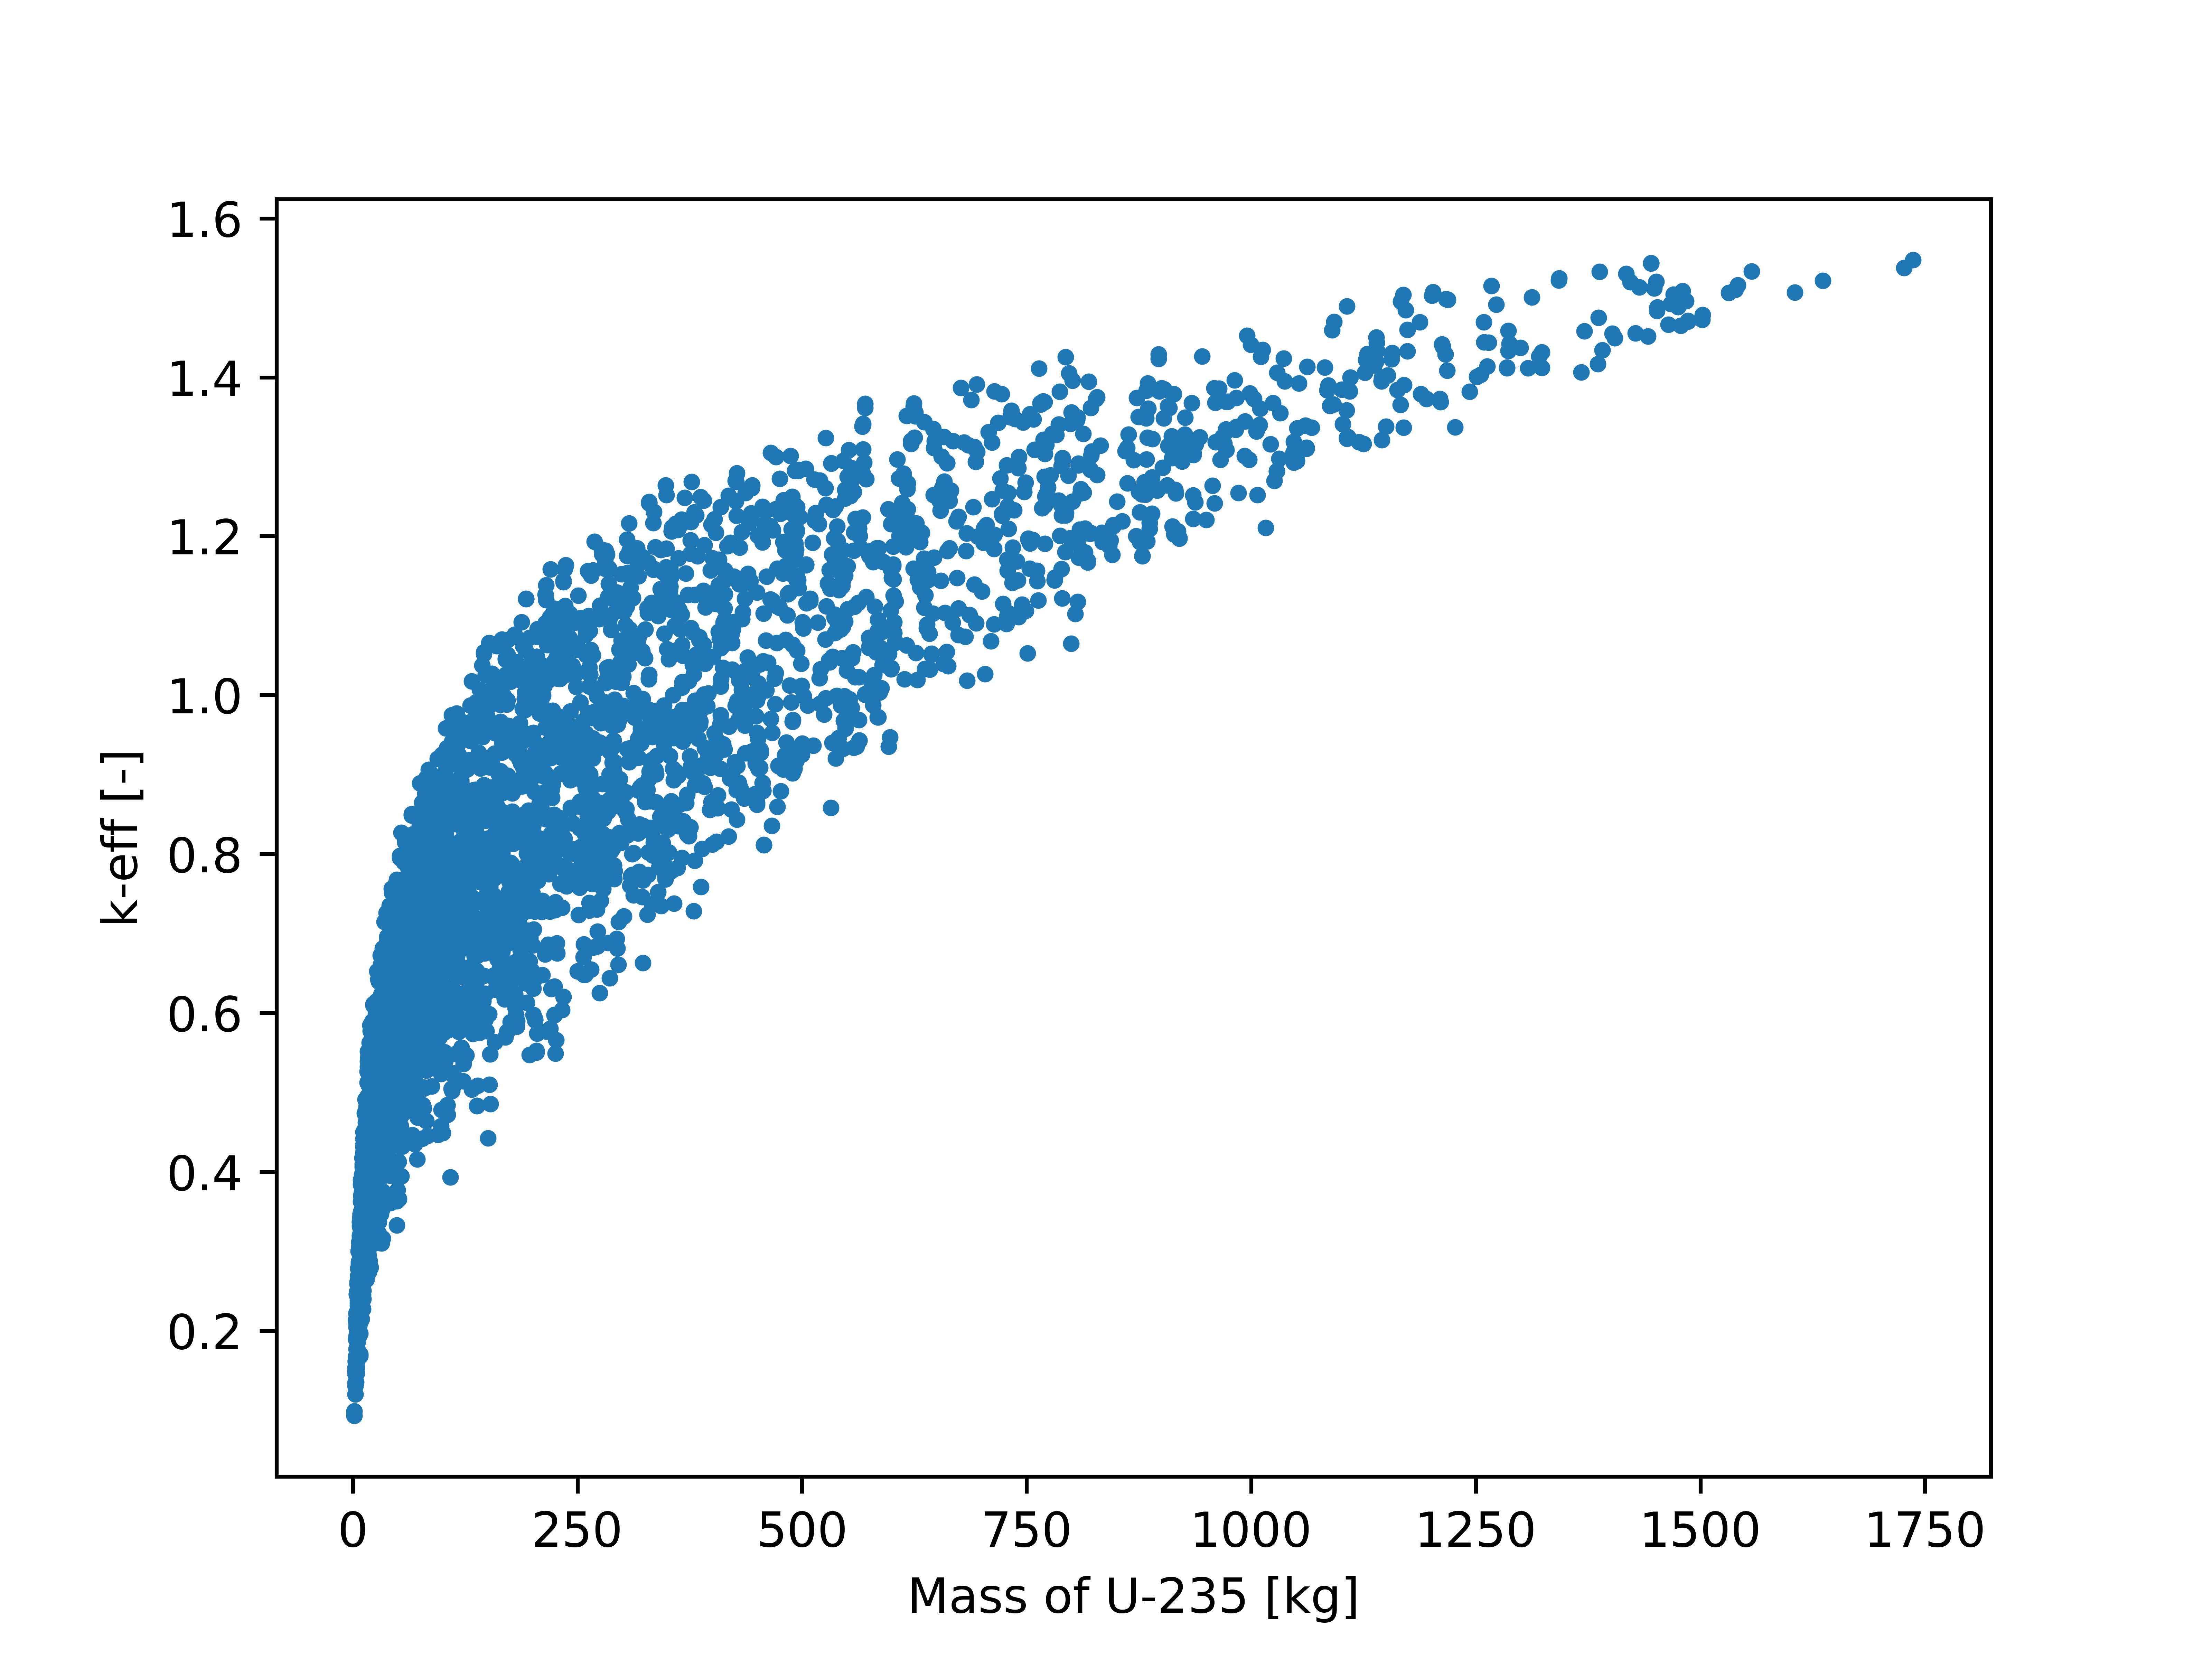
\includegraphics[width=3in]{../images/keff_vs_mass_235.png}
\caption{EOL \keff dependence on \uran mass}
\label{fig:eol_keff_vs_235_mass}
\end{figure}

This conclusion is useful for modeling a reactor's mass. Since EOL \keff is
dependent on \uran mass, for a fixed enrichment, EOL \keff can be modeled 
solely with reactor mass.

\section{Parametric Study Conclusion}
The purpose of this parametric study was to perform a rudimentry feature
selection. Feature selection is a technique used in machine learning and
statistics to select relevant variables (features) in a data set to simplify the
modeling of the data set. The parametric study helped identify key predictors
for the neutronic performance of a reactor design.

The figure of merit for neutronics performance was EOL \keff. The reactor must
sustain a fission chain reaction throughout the mission lifetime. In order to
ensure the reactor mass model generates a neutronically viable core, it was
necessary to determine on which input parameters EOL \keff is most strongly
dependent. To support this analysis, 3901 MCNP6.1 depletion calculations were
performed over a 5-dimensional sample space with Latin Hypercube Sampling
techniques to ensure even sampling. The conclusion of this work is that fissile
material mass is the most important parameter to predict EOL \keff. Another
important conclusion was that EOL \keff is relatively independent of thermal power. This
meant EOL \keff could be estimated as BOL \keff adjusted for minimal depletion.
This conclusion was useful to constrain reactor parameters and will be utilized
in Chapter \ref{ch:crit_radius} to generate a relationship between core fuel fraction
and a required core radius to ensure EOL \keff > 1.
